\documentclass{standalone}
\usepackage{tikz}
\usetikzlibrary{patterns, positioning}


\begin{document}
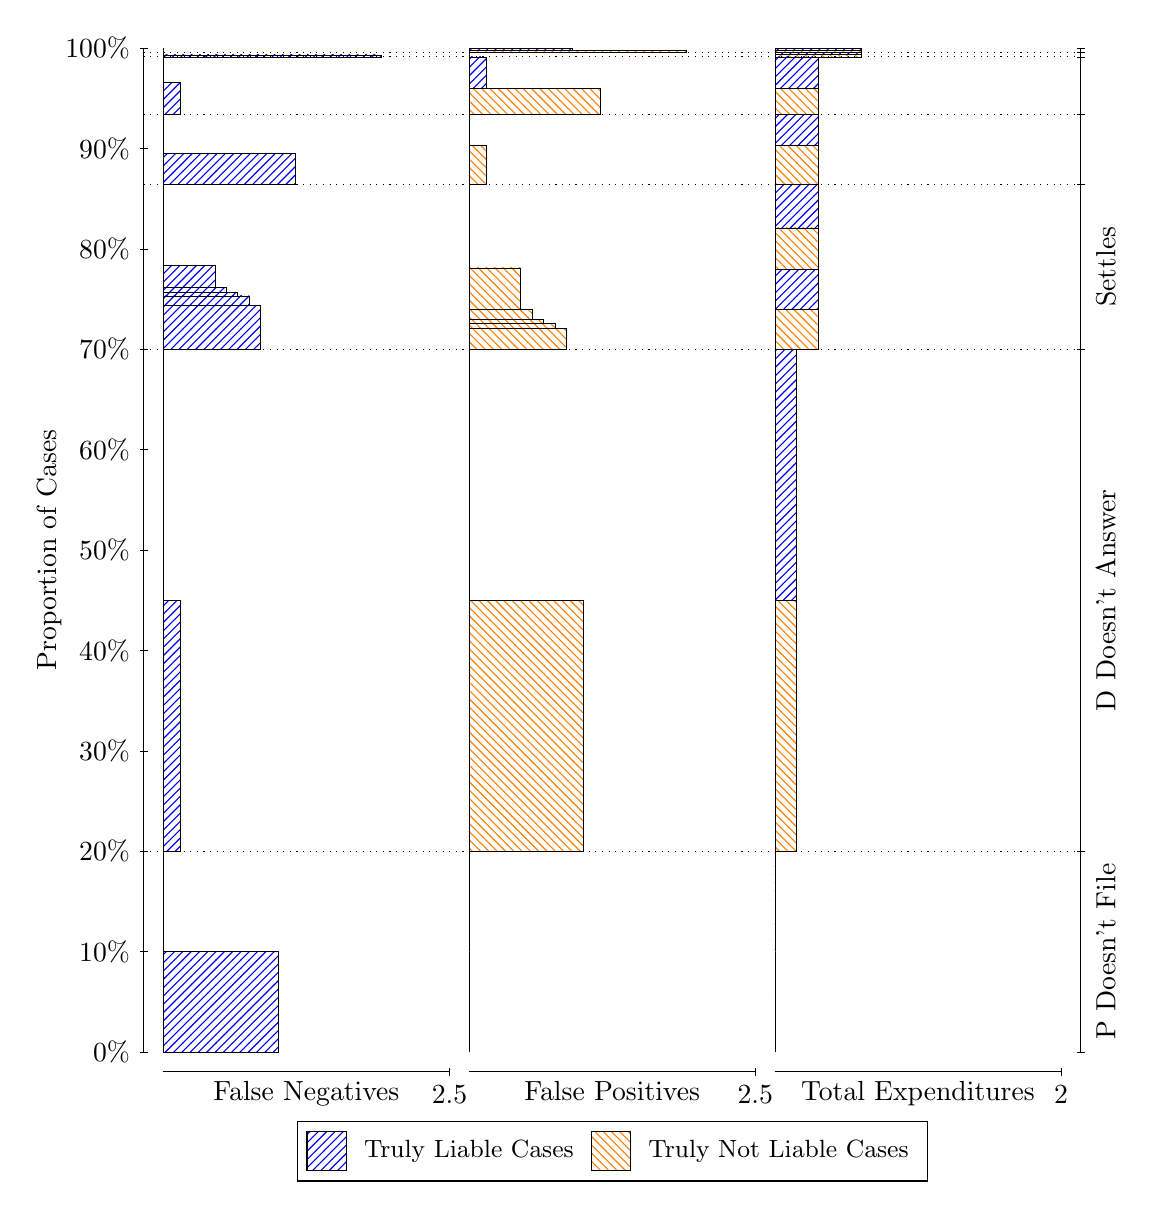
\begin{tikzpicture}
\draw[black, very thin] (1.5,1.75) -- (1.5,14.5);
\node[rotate=90, text=black, anchor=center] at (0.3, 8.125) {Proportion of Cases};
\draw[black, very thin] (1.45,1.75) -- (1.55,1.75);
\node[text=black, anchor=east] at (1.45, 1.75) {0\%};
\draw[black, very thin] (1.45,3.025) -- (1.55,3.025);
\node[text=black, anchor=east] at (1.45, 3.025) {10\%};
\draw[black, very thin] (1.45,4.3) -- (1.55,4.3);
\node[text=black, anchor=east] at (1.45, 4.3) {20\%};
\draw[black, very thin] (1.45,5.575) -- (1.55,5.575);
\node[text=black, anchor=east] at (1.45, 5.575) {30\%};
\draw[black, very thin] (1.45,6.85) -- (1.55,6.85);
\node[text=black, anchor=east] at (1.45, 6.85) {40\%};
\draw[black, very thin] (1.45,8.125) -- (1.55,8.125);
\node[text=black, anchor=east] at (1.45, 8.125) {50\%};
\draw[black, very thin] (1.45,9.4) -- (1.55,9.4);
\node[text=black, anchor=east] at (1.45, 9.4) {60\%};
\draw[black, very thin] (1.45,10.675) -- (1.55,10.675);
\node[text=black, anchor=east] at (1.45, 10.675) {70\%};
\draw[black, very thin] (1.45,11.95) -- (1.55,11.95);
\node[text=black, anchor=east] at (1.45, 11.95) {80\%};
\draw[black, very thin] (1.45,13.225) -- (1.55,13.225);
\node[text=black, anchor=east] at (1.45, 13.225) {90\%};
\draw[black, very thin] (1.45,14.5) -- (1.55,14.5);
\node[text=black, anchor=east] at (1.45, 14.5) {100\%};

\draw[black, very thin] (13.4,1.75) -- (13.4,14.5);
\draw[black, very thin] (13.35,1.75) -- (13.45,1.75);
\node[anchor=west] at (13.35, 1.75) {};
\draw[black, very thin] (13.35,4.3) -- (13.45,4.3);
\node[anchor=west] at (13.35, 4.3) {};
\draw[black, very thin] (13.35,10.675) -- (13.45,10.675);
\node[anchor=west] at (13.35, 10.675) {};
\draw[black, very thin] (13.35,12.771) -- (13.45,12.771);
\node[anchor=west] at (13.35, 12.771) {};
\draw[black, very thin] (13.35,13.656) -- (13.45,13.656);
\node[anchor=west] at (13.35, 13.656) {};
\draw[black, very thin] (13.35,14.388) -- (13.45,14.388);
\node[anchor=west] at (13.35, 14.388) {};
\draw[black, very thin] (13.35,14.444) -- (13.45,14.444);
\node[anchor=west] at (13.35, 14.444) {};
\draw[black, very thin] (13.35,14.5) -- (13.45,14.5);
\node[anchor=west] at (13.35, 14.5) {};

\draw[black, very thin, pattern color=blue, pattern=north east lines] (1.75,1.75) rectangle (3.2033,3.025);
\draw[black, very thin, pattern color=orange, pattern=north west lines] (1.75,3.025) rectangle (1.75,4.3);
\draw[black, very thin, pattern color=blue, pattern=north east lines] (1.75,4.3) rectangle (1.968,7.4875);
\draw[black, very thin, pattern color=orange, pattern=north west lines] (1.75,7.4875) rectangle (1.75,10.675);
\draw[black, very thin, pattern color=blue, pattern=north east lines] (1.75,10.675) rectangle (2.9853,11.23);
\draw[black, very thin, pattern color=blue, pattern=north east lines] (1.75,11.23) rectangle (2.84,11.353);
\draw[black, very thin, pattern color=blue, pattern=north east lines] (1.75,11.353) rectangle (2.6947,11.4);
\draw[black, very thin, pattern color=blue, pattern=north east lines] (1.75,11.4) rectangle (2.5493,11.456);
\draw[black, very thin, pattern color=blue, pattern=north east lines] (1.75,11.456) rectangle (2.404,11.736);
\draw[black, very thin, pattern color=orange, pattern=north west lines] (1.75,11.736) rectangle (1.75,12.771);
\draw[black, very thin, pattern color=blue, pattern=north east lines] (1.75,12.771) rectangle (3.4213,13.163);
\draw[black, very thin, pattern color=orange, pattern=north west lines] (1.75,13.163) rectangle (1.75,13.656);
\draw[black, very thin, pattern color=blue, pattern=north east lines] (1.75,13.656) rectangle (1.968,14.059);
\draw[black, very thin, pattern color=orange, pattern=north west lines] (1.75,14.059) rectangle (1.75,14.388);
\draw[black, very thin, pattern color=blue, pattern=north east lines] (1.75,14.388) rectangle (4.5113,14.414);
\draw[black, very thin, pattern color=orange, pattern=north west lines] (1.75,14.414) rectangle (1.75,14.444);
\draw[black, very thin, pattern color=orange, pattern=north west lines] (1.75,14.444) rectangle (1.75,14.469);
\draw[black, very thin, pattern color=blue, pattern=north east lines] (1.75,14.469) rectangle (1.75,14.5);
\draw[black, very thin, pattern color=orange, pattern=north west lines] (5.6333,1.75) rectangle (5.6333,3.025);
\draw[black, very thin, pattern color=blue, pattern=north east lines] (5.6333,3.025) rectangle (5.6333,4.3);
\draw[black, very thin, pattern color=orange, pattern=north west lines] (5.6333,4.3) rectangle (7.0867,7.4875);
\draw[black, very thin, pattern color=blue, pattern=north east lines] (5.6333,7.4875) rectangle (5.6333,10.675);
\draw[black, very thin, pattern color=orange, pattern=north west lines] (5.6333,10.675) rectangle (6.8687,10.938);
\draw[black, very thin, pattern color=orange, pattern=north west lines] (5.6333,10.938) rectangle (6.7233,11.005);
\draw[black, very thin, pattern color=orange, pattern=north west lines] (5.6333,11.005) rectangle (6.578,11.058);
\draw[black, very thin, pattern color=orange, pattern=north west lines] (5.6333,11.058) rectangle (6.4327,11.178);
\draw[black, very thin, pattern color=orange, pattern=north west lines] (5.6333,11.178) rectangle (6.2873,11.709);
\draw[black, very thin, pattern color=blue, pattern=north east lines] (5.6333,11.709) rectangle (5.6333,12.771);
\draw[black, very thin, pattern color=orange, pattern=north west lines] (5.6333,12.771) rectangle (5.8513,13.264);
\draw[black, very thin, pattern color=blue, pattern=north east lines] (5.6333,13.264) rectangle (5.6333,13.656);
\draw[black, very thin, pattern color=orange, pattern=north west lines] (5.6333,13.656) rectangle (7.3047,13.985);
\draw[black, very thin, pattern color=blue, pattern=north east lines] (5.6333,13.985) rectangle (5.8513,14.388);
\draw[black, very thin, pattern color=orange, pattern=north west lines] (5.6333,14.388) rectangle (5.6333,14.418);
\draw[black, very thin, pattern color=blue, pattern=north east lines] (5.6333,14.418) rectangle (5.6333,14.444);
\draw[black, very thin, pattern color=orange, pattern=north west lines] (5.6333,14.444) rectangle (8.3947,14.469);
\draw[black, very thin, pattern color=blue, pattern=north east lines] (5.6333,14.469) rectangle (6.9413,14.5);
\draw[black, very thin, pattern color=orange, pattern=north west lines] (9.5167,1.75) rectangle (9.5167,3.025);
\draw[black, very thin, pattern color=blue, pattern=north east lines] (9.5167,3.025) rectangle (9.5167,4.3);
\draw[black, very thin, pattern color=orange, pattern=north west lines] (9.5167,4.3) rectangle (9.7892,7.4875);
\draw[black, very thin, pattern color=blue, pattern=north east lines] (9.5167,7.4875) rectangle (9.7892,10.675);
\draw[black, very thin, pattern color=orange, pattern=north west lines] (9.5167,10.675) rectangle (10.062,11.178);
\draw[black, very thin, pattern color=blue, pattern=north east lines] (9.5167,11.178) rectangle (10.062,11.685);
\draw[black, very thin, pattern color=orange, pattern=north west lines] (9.5167,11.685) rectangle (10.062,12.216);
\draw[black, very thin, pattern color=blue, pattern=north east lines] (9.5167,12.216) rectangle (10.062,12.771);
\draw[black, very thin, pattern color=orange, pattern=north west lines] (9.5167,12.771) rectangle (10.062,13.264);
\draw[black, very thin, pattern color=blue, pattern=north east lines] (9.5167,13.264) rectangle (10.062,13.656);
\draw[black, very thin, pattern color=orange, pattern=north west lines] (9.5167,13.656) rectangle (10.062,13.985);
\draw[black, very thin, pattern color=blue, pattern=north east lines] (9.5167,13.985) rectangle (10.062,14.388);
\draw[black, very thin, pattern color=orange, pattern=north west lines] (9.5167,14.388) rectangle (10.607,14.418);
\draw[black, very thin, pattern color=blue, pattern=north east lines] (9.5167,14.418) rectangle (10.607,14.444);
\draw[black, very thin, pattern color=orange, pattern=north west lines] (9.5167,14.444) rectangle (10.607,14.469);
\draw[black, very thin, pattern color=blue, pattern=north east lines] (9.5167,14.469) rectangle (10.607,14.5);
\draw[black, dotted] (1.5,4.3) -- (13.4,4.3);
\draw[black, dotted] (1.5,10.675) -- (13.4,10.675);
\draw[black, dotted] (1.5,12.771) -- (13.4,12.771);
\draw[black, dotted] (1.5,13.656) -- (13.4,13.656);
\draw[black, dotted] (1.5,14.388) -- (13.4,14.388);
\draw[black, dotted] (1.5,14.444) -- (13.4,14.444);
\draw[black, very thin] (1.75,1.5) -- (5.3833,1.5);
\node[text=black, anchor=north] at (3.5667, 1.5) {False Negatives};
\draw[black, very thin] (5.3833,1.45) -- (5.3833,1.55);
\node[text=black, anchor=north] at (5.3833, 1.45) {2.5};

\draw[black, very thin] (5.6333,1.5) -- (9.2667,1.5);
\node[text=black, anchor=north] at (7.45, 1.5) {False Positives};
\draw[black, very thin] (9.2667,1.45) -- (9.2667,1.55);
\node[text=black, anchor=north] at (9.2667, 1.45) {2.5};

\draw[black, very thin] (9.5167,1.5) -- (13.15,1.5);
\node[text=black, anchor=north] at (11.333, 1.5) {Total Expenditures};
\draw[black, very thin] (13.15,1.45) -- (13.15,1.55);
\node[text=black, anchor=north] at (13.15, 1.45) {2};

\node[text=black, centered, rotate=90] at (13.72, 3.025) {P Doesn't File};
\node[text=black, centered, rotate=90] at (13.72, 7.4875) {D Doesn't Answer};
\node[text=black, centered, rotate=90] at (13.72, 11.723) {Settles};





\draw (7.449999999999999,1.5) node[draw=none] (baseCoordinate) {};
\begin{scope}[align=center]
        \matrix[scale=0.5, draw=black, below=0.5cm of baseCoordinate, nodes={draw}, column sep=0.1cm]{
            \node[rectangle, draw, minimum width=0.5cm, minimum height=0.5cm, pattern color=blue, pattern=north east lines] {}; &
            \node[draw=none, font=\small, text=black] (B) {Truly Liable Cases}; &
            \node[rectangle, draw, minimum width=0.5cm, minimum height=0.5cm, pattern color=orange, pattern=north west lines] {}; &
            \node[draw=none, font=\small, text=black] (B) {Truly Not Liable Cases}; \\
            };
\end{scope}

\end{tikzpicture}
\end{document}